\chapter{Structural view}

\section{Introduction}
This chapter describes the structural architecture of the system in a top down approach.\\
The blocks are derived from previous documentation.


\section{System overview}
The system consist of a central data unit and n number of sensors.
\begin{figure}[hbpt]
\centering
\includegraphics[width=.9\textwidth]{billeder/systembdd}
\caption{System block definition diagram}
\label{systembdd}
\end{figure}

\subsection{Block responsibility}
\subsubsection{CDU}
The CDU contacts each sensor to collect the data values. This is then stored for later extraction.

\subsubsection{Sensor n}
The sensor measures a physical or biometric parameter such as temperature, movement, humidity etc.

\section{Detailed block overview}
Below are detailed figures for each block in the system.\\
The blocks in the figures are conceptual blocks and most of the consist of both software and hardware.\\
All blocks are essential to full fill the functionality and requirements of the system.

\subsection{CDU}

\begin{figure}[hbpt]
\centering
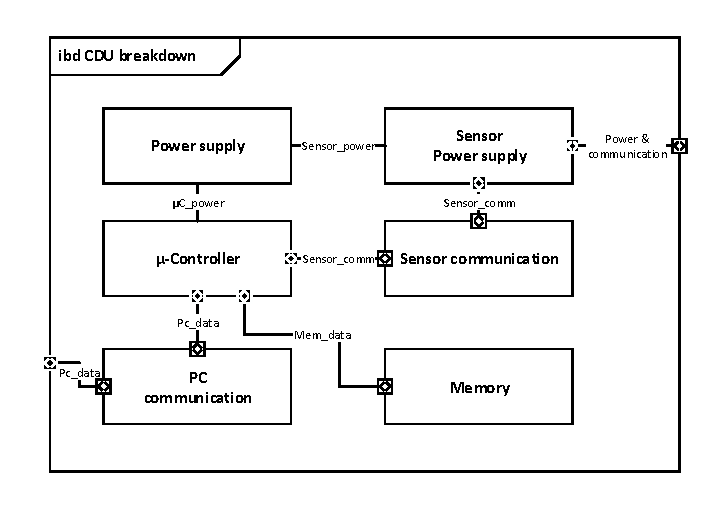
\includegraphics[width=.9\textwidth]{billeder/CDU_IBD}
\caption{Internal Block Diagram of the CDU}
\label{CDU_IBD}
\end{figure}

\subsection{Sensor n}

\begin{figure}[hbpt]
\centering
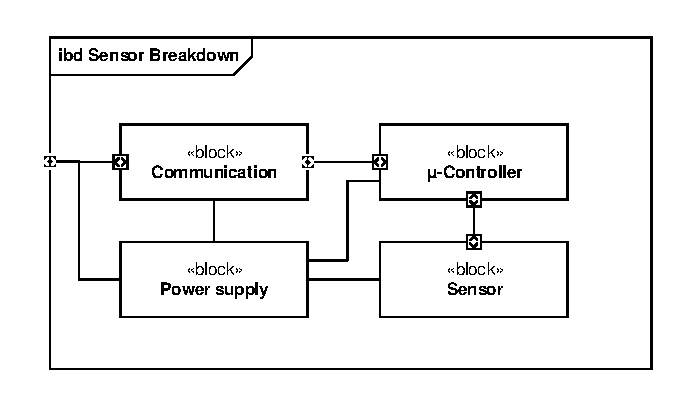
\includegraphics[width=.9\textwidth]{billeder/Sensor_IBD}
\caption{Internal Block Diagram of the sensor}
\label{Sensor_IBD}
\end{figure}

